% !TEX program = pdflatex
% !TEX encoding = UTF-8
% !TEX spellcheck = en_US
\documentclass[12pt]{article}

\usepackage[margin=1in]{geometry}
\usepackage[utf8]{inputenc}
\usepackage{amsmath,amsthm,amssymb}
\usepackage{graphicx}
\usepackage{hyperref} % Uso de links
\usepackage[version=4]{mhchem}
\usepackage{siunitx}
\usepackage{enumerate}
\usepackage{titlesec}
\usepackage{booktabs}
\usepackage{bm}
\usepackage[autostyle]{csquotes}
\usepackage{xcolor}

\titleformat{\subsection}
  {\normalfont\large\bfseries}{}{0em}{}

\setlength{\parindent}{0em}

\begin{document}

% --------------------------------------------------------------
%                         Start here
% --------------------------------------------------------------

\title{Mechanical Properties of Materials (MSAE 4215), Spring 2019\\ Homework 2 Solutions}
\author{Qi Zhang}
\date{\today}

\maketitle

\tableofcontents
\listoffigures

\section{Problems}
{\color{red} \textbf{Notice:} All updated contents will be colored in red!}
\subsection{2.1}
Consider a solid cylinder, radius $R$, length $l$, density $\rho$ standing up on its end,
so that its total height (in $x_3$) above the pavement is $l$. Assume normal stresses only.
Derive an expression for the stress in the material as a function of $x_3$, and
plot $\sigma_{33}(x_3)$. How tall can a solid column of concrete ($\rho = \SI{2}{\gram\per\cubic\centi\meter}$)
be made before the maximum shear stress exceeds the critical shear stress for
fracture, $\tau_c = \SI{10}{\mega\pascal}$? Take $\sigma_{33} \sim \tau_\text{max}$ at fracture.
(Recall that the total forces exerted on the body have to sum to zero.)

\textbf{Solution:}

At equilibrium
\begin{equation}
	0 = \sum_{j}\frac{\partial \sigma_{ij}}{\partial x_j} + g_{i}.
\end{equation}
The only body force present is due to the weight of the cylinder. The body force per unit volume is
\begin{equation}
	g_3 = \frac{m g}{V} = \rho g.
\end{equation}
Considering the $x_3$ direction only
\begin{equation}
	0 = \frac{\partial \sigma_{33}}{\partial x_3} + g_{3}.
\end{equation}
Rearranging and integrating yields
\begin{align}
	\frac{ d\sigma_{33} }{ d x_3 } & = -\rho g,         \\
	\sigma_{33}(x_3)               & = -\rho g x_3 + C,
\end{align}
where $C$ is a constant to be determined.
We can solve for the constant of integration by using the ``initial condition"
that the stress at the top of the
cylinder is zero since there are no tractive forces present at the free-end. Thus
\begin{align}
	\sigma_{33}(L) = 0 & = -\rho g L + C,    \\
	C                  & = \rho g L,         \\
	\sigma_{33}(x_3)   & = \rho g (L - x_3).
\end{align}
From this expression we can see
the maximum stress occurs when $x_3 = 0$.
Thus, we can solve for $l$, by setting $\sigma_{33}$ to $\tau_c$ at $x_3 = 0$. Thus
\begin{equation}
	l = \frac{\sigma_{33}}{\rho g} \approx \SI{510}{\meter}.
\end{equation}

\subsection{2.2}
Consider a small sphere of \ce{NdFeB} permanent magnet material in a large,
uniform, superconducting magnetic field of \SI{10}{\tesla}. If its magnetization $M$
is initially orthogonal to the applied field $\mu_0 H$ when the field is (instantaneously)
turned on, does the sphere shatter? Take $\tau_c = \SI{50}{\mega\pascal}$? and
$\mu_0 M_s = \SI{0.5}{\tesla}$.

\textbf{Solution:}

We can compute the body torque using
\begin{equation}
	\bm{G} = -\mu_0 \bm{M} \times \bm{H}.
\end{equation}
Since
\begin{equation}
	{\color{red} \bm{B} = \mu_{0} (\bm{H} + \bm{M}) \approx \mu_{0} \bm{H},}
\end{equation}
And the magnetic field, $\bm{B}$, is initially orthogonal to the magnetization, $\bm{M}$,
of the sphere, the magnitude of $\bm{G}$ is
\begin{equation}
	G = \mu_0 M_s \frac{B}{\mu_0} = \frac{0.5 \times 10}{4 \pi \times 10^{-7}} \si{\pascal} \approx \SI{3.98}{\mega\pascal} < \SI{50}{\mega\pascal},
\end{equation}
where $\mu_0$ is the vacuum permeability.
So the sphere will not shatter.

\subsection{2.3}
There is a longstanding proposal for a space elevator, as pictured in
Figure $2.5$. If a mass $M$ can be attached to a long cable, length $l$, and $l \gg R$,
where $R$ is the radius of the earth, gravity is less strong than the centrifugal force,
the cable might be supported.
1) Assume that there is no counterweight ($M = 0$). For a cable density $\rho$,
how long does the cable need to be for it to stand up (i.e. all sections in tension)?
Estimate $l/R$ for a density of $\rho = \SI{2}{\gram\per\cubic\centi\meter}$,
appropriate for carbon fiber. 2) Plot the stress in the cable, and calculate the
maximum stress.

\textbf{Solution:}

An introduction from Wikipedia:
\blockquote{
	An Earth space elevator cable rotates along with the rotation of the Earth.
	Therefore the cable, and objects attached to it, would experience upward centrifugal
	force in the direction opposing the downward gravitational force.
	The higher up the cable the object is located, the less the gravitational pull of the Earth,
	and the stronger the upward centrifugal force due to the rotation,
	so that more centrifugal force opposes less gravity.
	The centrifugal force and the gravity are balanced at geosynchronous equatorial orbit (GEO).
	Above GEO, the centrifugal force is stronger than gravity, causing objects attached to the cable there to pull upward on it.

	The net force for objects attached to the cable is called the apparent gravitational field. The apparent gravitational field for attached objects is the (downward) gravity minus the (upward) centrifugal force. The apparent gravity experienced by an object on the cable is zero at GEO, downward below GEO, and upward above GEO.
}
But now we do not have a counterweight attached at the end ($M = 0$), so the counterweight is the cable itself.
At each point on the cable (distance $x$ from the Earth surface), we make use of
\begin{equation}\label{eq:sgg}
	\frac{\partial \sigma}{\partial x} = \frac{G M \rho}{(R + x)^2} - \rho \omega^2 (R + x),
\end{equation}
where
\begin{equation}
	\frac{G M \rho}{(R + x)^2}
\end{equation}
is the Newton's universal law of gravitation, and
\begin{equation}
	\rho \omega^2 (R + x)
\end{equation}
is the magnitude of the centrifugal force.
We are assuming $\sigma > 0$ for tension, and $\sigma < 0$ for contraction. And below GEO the gravity is larger than
the centrifugal force, above GEO the first is smaller.

Integrate \eqref{eq:sgg}, we get
\begin{equation}
	\sigma(x) = -\frac{\rho \omega^2 (R + x)^2}{2} - \frac{ G M \rho }{ R + x } + C,
\end{equation}
where $C$ is a constant to be determined.
Once again we can solve for the constant of integration by using the ``initial condition" that the stress at the top of the space elevator is $0$ since there are no tractive forces present at the free-end. Thus:
\begin{equation}
	\sigma(l) = 0,
\end{equation}
for a cable with length $l$.
Then
\begin{equation}\label{eq:sgsolu}
	\sigma(x) = G \rho M \bigg( \frac{1}{R + l} - \frac{1}{R + x}\bigg) + \frac{ \rho \omega^2 }{ 2 } \big( (R + l)^2 - (R + x)^2 \big),
\end{equation}
We need one more condition in order to solve for $l$. We cannot say much about the stress at the base of the space elevator, \textit{a priori}. However, we can use the condition that we require all sections of the cable to be in tension.

If we plot the \eqref{eq:sgsolu} with different initial solutions $\sigma(0) = \sigma_0$, we get figure \ref{fig:stress}.
\begin{figure}[h]
	\centering
	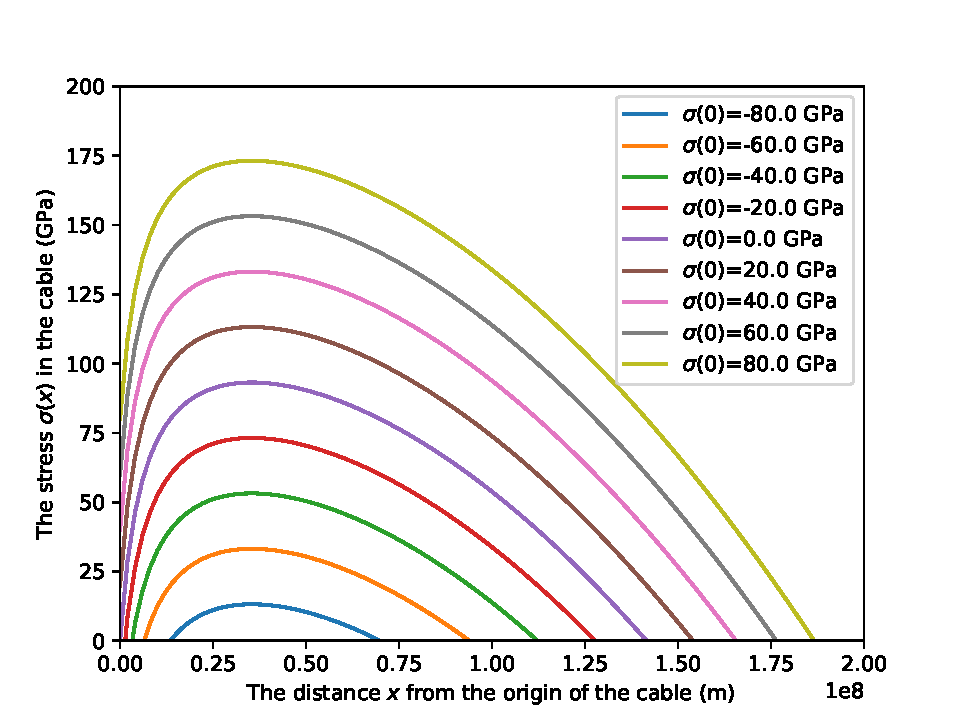
\includegraphics[width=0.8\linewidth]{images/stress.pdf}
	\caption{Stress vs distance in the cable. Note that $x$ has a scale of $10^8$.}
	\label{fig:stress}
\end{figure}

Clearly we observe, if we set $\sigma(0) < 0$, we will have a large range of $x$, on which $\sigma(x) < 0$. So
we should force $\sigma \ge 0$, i.e., pick those lines no lower than the purple one.

For the blue line and lines above, we have a cutoff length $x_\text{max}$, s.t.,
\begin{equation}
	\sigma(x) < 0 \text{ for } x > x_\text{max},
\end{equation}
based on the same reason.
Among those lines, the blue line has the shortest length to the cable, so one solution is
\begin{equation}
	\sigma(0) = 0 \Rightarrow l = \SI{1.473e8}{\meter}.
\end{equation}
You can derive this by putting $\sigma(0) = 0$ into \eqref{eq:sgsolu}.
The maximum stress, of course, is when
\begin{equation}
	\bigg( \frac{ \partial \sigma }{ \partial x } \bigg)_{x=x_0} = 0 = \frac{G M \rho}{(R + x_0)^2} - \rho \omega^2 (R + x_0),
\end{equation}
we get
\begin{equation}
	x_0 \approx \SI{35786}{\kilo\meter} \approx 5.6 R.
\end{equation}
Note that this value is not related to $\rho$, i.e., the material of the cable, because it is just the geostationary orbit (GEO)!

Parameters we used:
$\rho = \SI{2000}{\kilogram\per\cubic\meter}$,
%$\omega=2\pi/24/3600=7.27 \times 10^{−5}$ s$^{-1}$,
$G = 6.67 \times 10^{-11}$ m$^3$/(kg s${^2}$), $R = \SI{6.4e6}{\meter}$,
Earth mass $M = \SI{5.79e24}{\kilogram}$.

\begin{figure}[h]
	\centering
	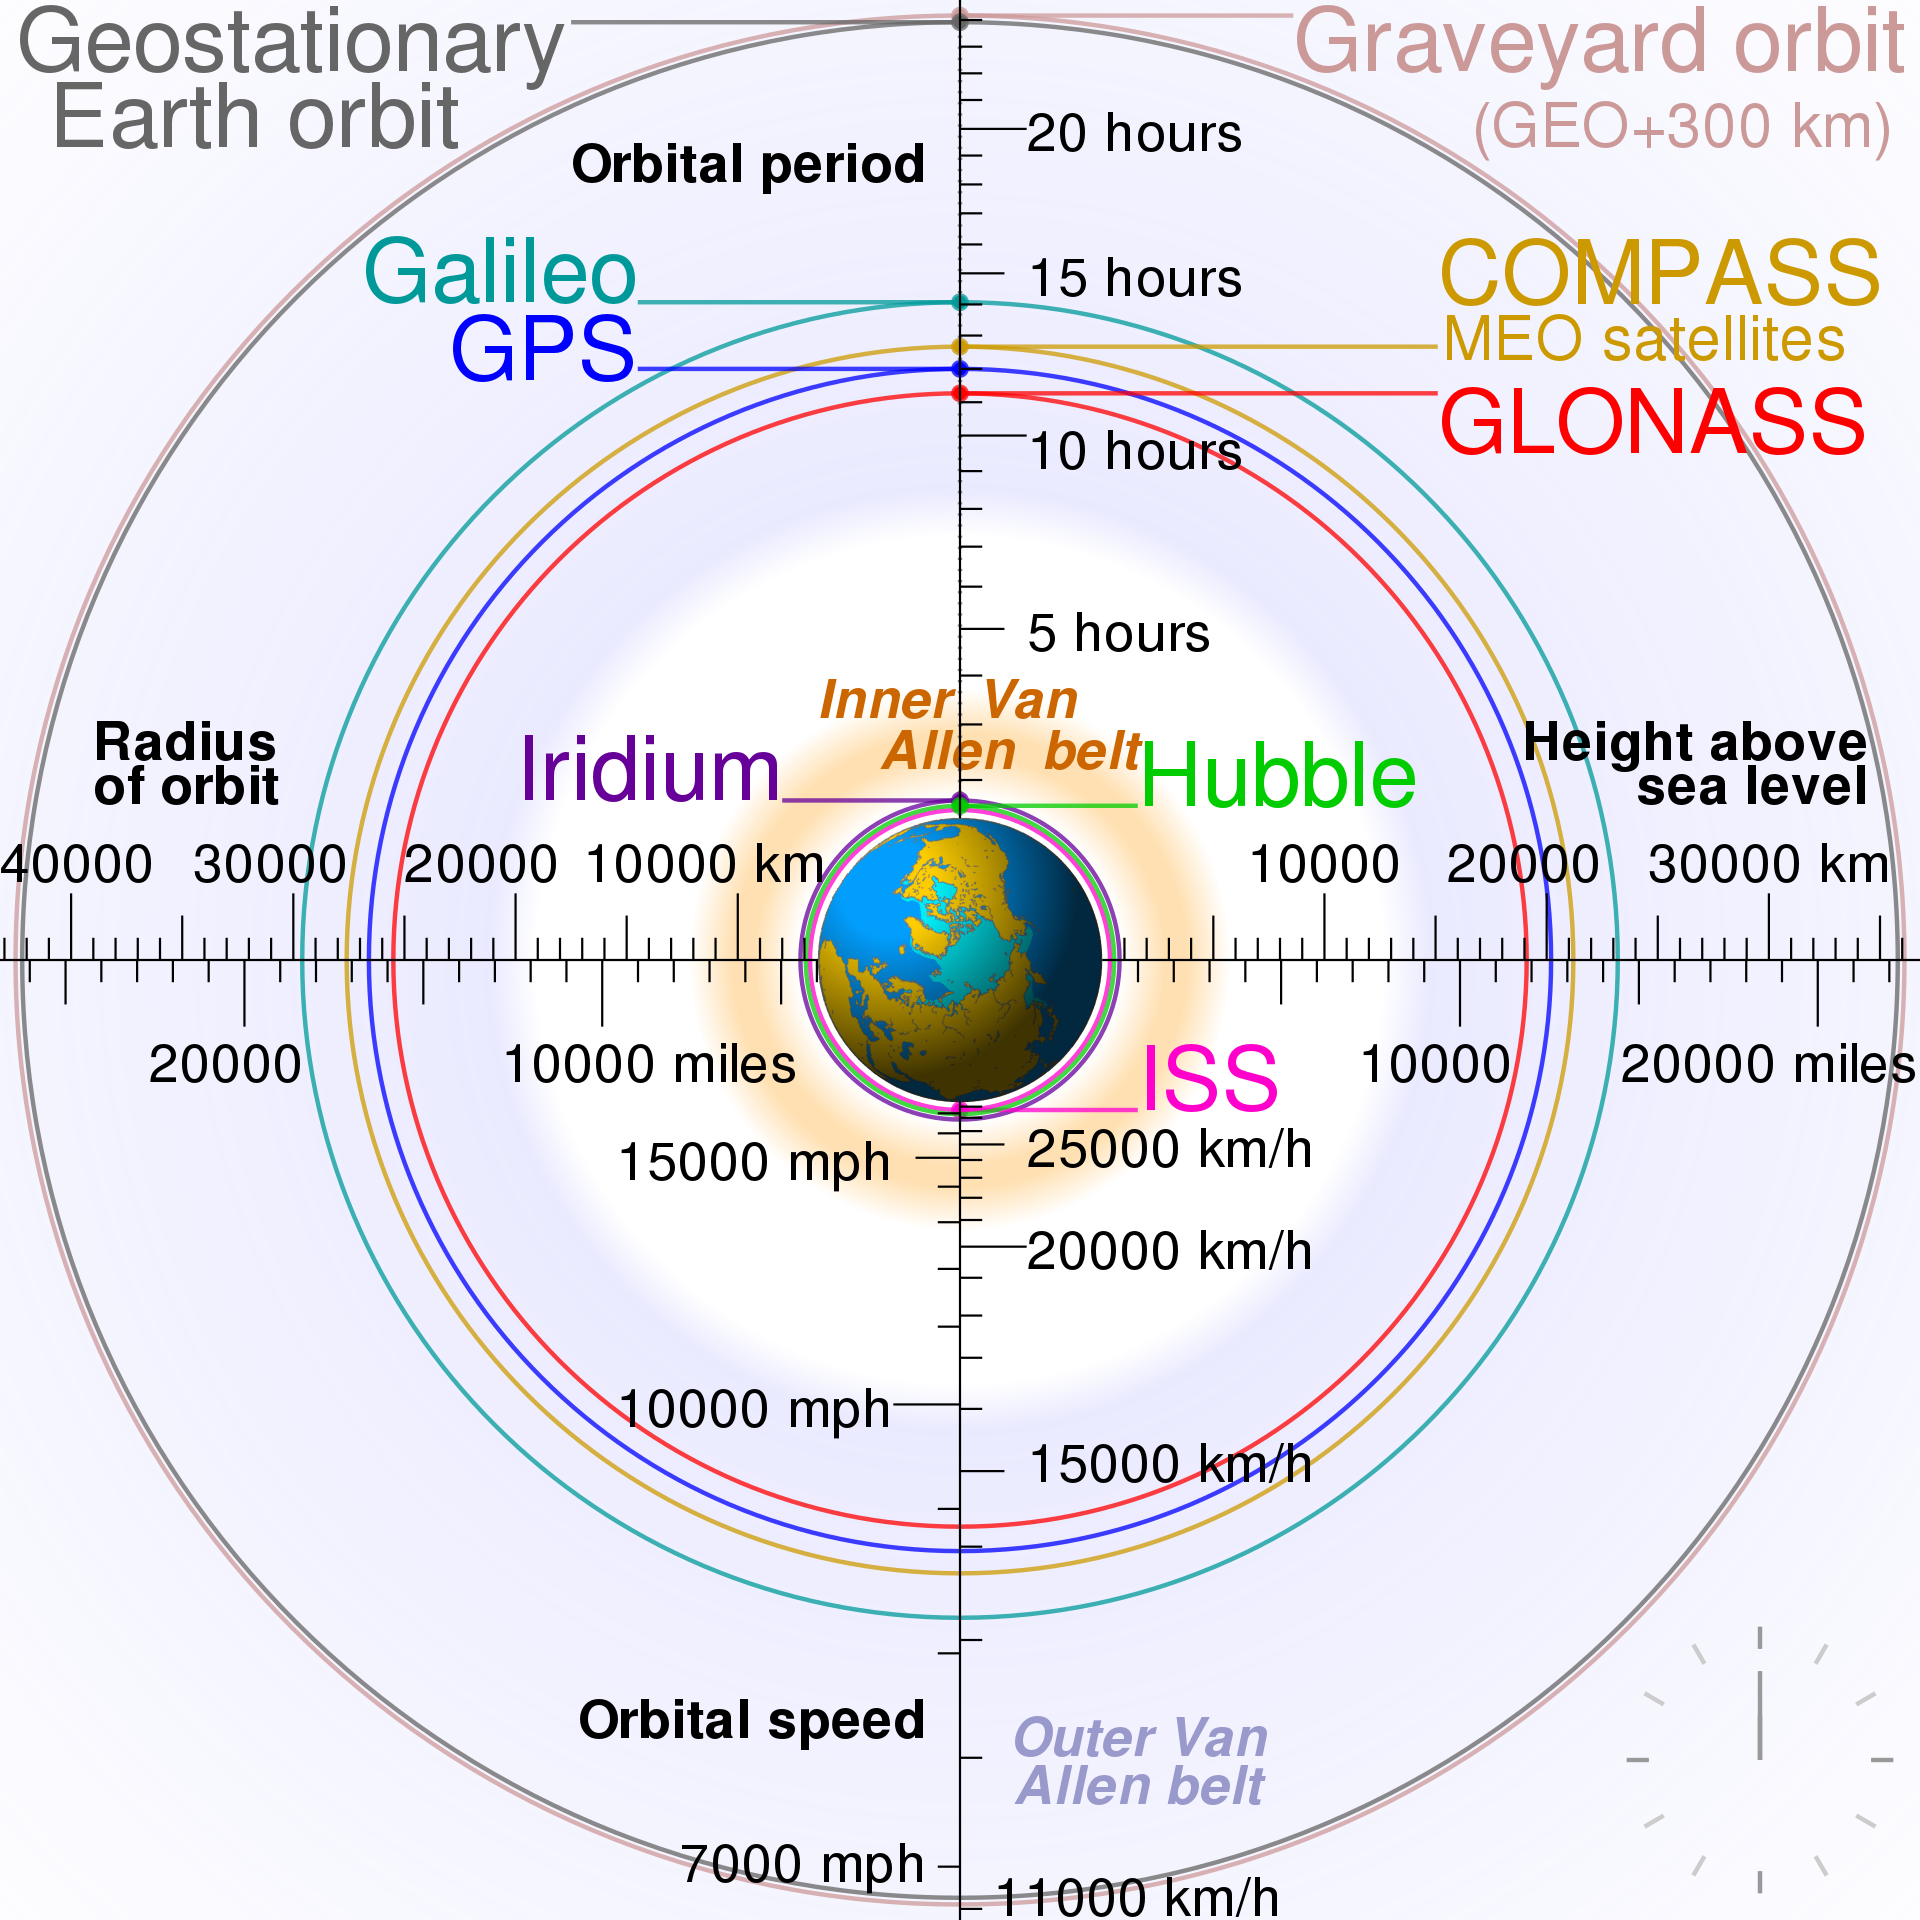
\includegraphics[width=0.7\linewidth]{images/GEO}
	\caption{GEO from \url{https://en.wikipedia.org/wiki/Geostationary_orbit}}
	\label{fig:geo}
\end{figure}

The single-walled or multi-walled carbon nanotubes are expected to have an ideal strength of about
\SI{100}{\giga\pascal},\cite{pugno2006strength}
so maybe we can verify that $\sigma(0) = 0$ is a possible choice since its maximum stress is not beyond \SI{100}{\giga\pascal}.
Though an optimized cable design must consider a uniform tensile stress profile rather than a constant
cross-section area.\cite{pugno2006strength} What we considered now is just a simple example problem.

\subsection{3.1}
For a solid cylinder under uniaxial normal stress along $x_2$, $\sigma_{22} = \sigma$,
\begin{itemize}
	\item Find the shear stress $\sigma_{\alpha\beta}$ for orthonormal ($\alpha$, $\beta$, $x_3$)
	      and $\alpha$, $\beta$ rotated by $\theta_3$ about $x_3$ with respect to $x_1$, $x_2$.

	      \textbf{Solution:}

	      We can represent the rotation around a single axis as a forward transformation of a rank two tensor use
	      dummy suffix notation:
	      \begin{equation}
		      \sigma_{\alpha\beta}' = a_{\alpha k} a_{\beta j} \sigma_{kj}.
	      \end{equation}
	      As a reminder, we keep the indices close for a transformation from old to new (a forward transformation).
	      Since $\sigma_{22} = \sigma$ is the only non-zero value of $\sigma_{kl}$:
	      \begin{equation}
		      \sigma_{\alpha\beta}' = a_{\alpha 2} a_{\beta 2} \sigma_{22} = \sin(\theta_3) \cos(\theta_3) \sigma = \frac{\sin(2\theta_3)}{2} \sigma,
	      \end{equation}
	      since
	      \begin{equation}
		      \sin(x) \cos(x) = \frac{\sin(2x)}{2}.
	      \end{equation}
	\item Find the shear stress $\sigma_{\alpha\beta}$ for a general rotation $\theta$,
	      and show that it is maximum for $\theta = \pi/4$.

	      \textbf{Solution:}
	      \begin{figure}[h]
		      \centering
		      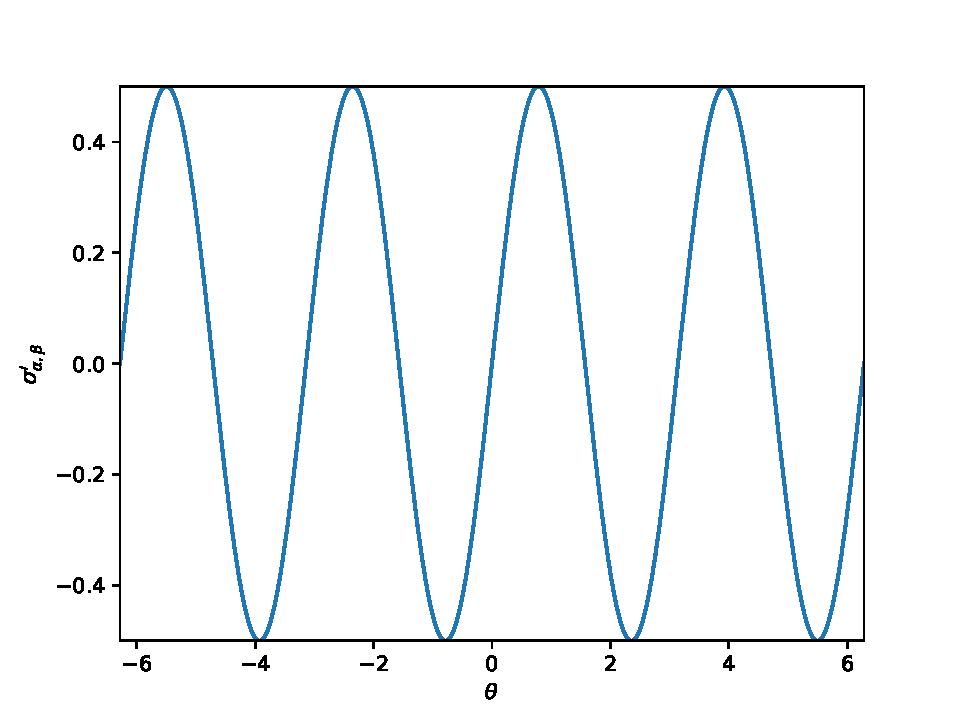
\includegraphics[width=0.7\linewidth]{images/sin}
		      \caption{$\sigma_{\alpha\beta}'$ vs $\theta$.}
		      \label{fig:sin}
	      \end{figure}

	      Using our answer from the last question, for a general rotation of $\theta$,
	      \begin{equation}
		      \sigma_{\alpha\beta}' = \frac{\sin(2\theta)}{2} \sigma,
	      \end{equation}
	      We can show either by evaluating
	      \begin{equation}
		      \frac{d\sigma_{\alpha\beta}'}{d \theta} = \cos(2 \theta) \sigma,
	      \end{equation}
	      or via inspection that when $\theta = \pi / 4$, then
	      \begin{equation}
		      \sigma_{\alpha\beta}' = \sigma / 2
	      \end{equation}
	      is at a maximum.
\end{itemize}


\subsection{3.2}
Consider the following biaxial stress state: $\sigma_{11} = \SI{300}{\mega\pascal}$,
$\sigma_{22} = \SI{100}{\mega\pascal}$, $\sigma_{12} = \SI{100}{\mega\pascal}$,
with $\alpha$, $\beta$ axes defined as before
\begin{itemize}
	\item Determine the rotation $\theta_3$ such that $\alpha$, $\beta$ are principal axes.

	      \textbf{Solution:}

	      For the this biaxial stress state we will make use of Mohr’s circle. It’s a very useful construct when
	      considering rotations about a single axis. We can find the principal axis using Eq. $(3.63)$:
	      \begin{equation}
		      \tan(2\theta_3) = \frac{2 \sigma_{12}}{\sigma_{11} - \sigma_{22}}.
	      \end{equation}
	      Thus
	      \begin{equation}
		      \theta_3 = \frac{1}{2} \arctan \Big( \frac{2 \sigma_{12}}{\sigma_{11} - \sigma_{22}} \Big) = \frac{\pi}{8}.
	      \end{equation}

	\item Determine the principal stresses $\sigma_{\alpha\alpha}$, $\sigma_{\beta\beta}$.

	      \textbf{Solution:}

	      Likewise the principal stress are determined via Eqs. (3.65), (3.66), (3.67).
	      \begin{equation}
		      R = \sqrt{\sigma_{12}^2 + \Big( \frac{\sigma_{11} - \sigma_{22}}{2} \Big)^2} = \SI[parse-numbers = false, number-math-rm = \ensuremath]{100 \sqrt{2}}{\mega\pascal}.
	      \end{equation}
	      \begin{equation}
		      C = \bigg( \frac{\sigma_{11} + \sigma_{22}}{2} \bigg) = \SI{200}{\mega\pascal}.
	      \end{equation}
	      \begin{align}
		      \sigma_{\alpha\alpha} & = C + R = \SI[parse-numbers = false, number-math-rm = \ensuremath]{100 \sqrt{2} + 200}{\mega\pascal},  \\
		      \sigma_{\beta\beta}   & = C - R = \SI[parse-numbers = false, number-math-rm = \ensuremath]{-100 \sqrt{2} + 200}{\mega\pascal}.
	      \end{align}

	\item Determine the $\theta_3$ for maximum in-plane shear and the magnitude of the maximum $\sigma_{\alpha\beta}$.

	      \textbf{Solution:}

	      A rotation of $2 \theta_3 = \frac{\pi}{2}$
	      from the principal axes results in a maximal shear state. Thus, from the original
	      axis a rotation of $-\frac{ \pi }{ 8 }$ or $\frac{ 3\pi }{ 8 }$ will result in a maximum shear state.
	      The magnitude is:
	      \begin{equation}
		      \sigma_{\alpha\beta}^\text{max} = R = \SI[parse-numbers = false, number-math-rm = \ensuremath]{100 \sqrt{2}}{\mega\pascal}.
	      \end{equation}
\end{itemize}


\subsection{3.3}
Take the following stress tensor:
\begin{equation}
	[\sigma] = \begin{bmatrix}
		0           & \sigma_{12} & 0           \\
		\sigma_{12} & \sigma_{22} & \sigma_{23} \\
		0           & \sigma_{23} & 0
	\end{bmatrix}
\end{equation}
Note that no principal stress axis is known \textit{a priori}.
\begin{itemize}
	\item Write an expression for the principal stresses. How many nonzero principal stresses are there?

	      \textbf{Solution:}

	      Here we need to solve the eigenvalue problem
	      \begin{equation}
		      [\sigma] \begin{bmatrix}
			      x_1 \\
			      x_2 \\
			      x_3
		      \end{bmatrix} = \lambda
		      \begin{bmatrix}
			      x_1 \\
			      x_2 \\
			      x_3
		      \end{bmatrix}.
	      \end{equation}
	      Which is equivalent to solving $\lambda$ from
	      \begin{equation}
		      \begin{vmatrix}
			      -\lambda    & \sigma_{12}           & 0           \\
			      \sigma_{12} & \sigma_{22} - \lambda & \sigma_{23} \\
			      0           & \sigma_{23}           & -\lambda
		      \end{vmatrix} = 0.
	      \end{equation}
	      We can use expansion by cofactors, along the first row to evaluate the determinant:
	      \begin{align}
		      -\lambda (-1)^{1+1}
		      \begin{vmatrix}
			      \sigma_{22} - \lambda & \sigma_{23} \\
			      \sigma_{23}           & -\lambda
		      \end{vmatrix}
		      + \sigma_{12} (-1)^{1+2}
		      \begin{vmatrix}
			      \sigma_{12} & \sigma_{23} \\
			      0           & -\lambda
		      \end{vmatrix}
		      + 0 (-1)^{1+3}
		      \begin{vmatrix}
			      \sigma_{12} & \sigma_{22} - \lambda \\
			      0           & \sigma_{23}
		      \end{vmatrix}                                                       & = 0, \\
		      -\lambda \Big( \lambda^2 - \lambda \sigma_{22} - (\sigma_{23}^2 + \sigma_{12}^2) \Big) & = 0.
	      \end{align}
	      Thus, the principal stresses are:
	      \begin{align}\label{eq:lambdas}
		      \lambda_1 & = 0,                                                                                   \\
		      \lambda_2 & = \frac{ \sigma_{22} + \sqrt{\sigma_{22}^2 + 4(\sigma_{12}^2 + \sigma_{23}^2)} }{ 2 }, \\
		      \lambda_3 & = \frac{ \sigma_{22} - \sqrt{\sigma_{22}^2 + 4(\sigma_{12}^2 + \sigma_{23}^2)} }{ 2 }.
	      \end{align}
	      Two of them are non-zero.

	\item Verify that the dilation $\Delta$ is invariant on transforming to the principal axes.

	      \textbf{Solution:}

	      \begin{equation}
		      \Delta = \lambda_1 + \lambda_2 + \lambda_3 = 0 + \sigma_{22} + 0.
	      \end{equation}
	\item Solve the principal stresses for $\sigma_{22} = \SI{200}{\mega\pascal}$,
	      $\sigma_{12} = \sigma_{23} = \sqrt{2} \cdot \SI{100}{\mega\pascal} \sim \SI{141}{\mega\pascal}$.

	      \textbf{Solution:}

	      By substituting numbers into \eqref{eq:lambdas},
	      \begin{align}
		      \lambda_1 & = 0,                         \\
		      \lambda_2 & = \SI{323.1}{\mega\pascal},  \\
		      \lambda_3 & = \SI{-123.1}{\mega\pascal}.
	      \end{align}
	\item Determine the principal axes. If there is plane stress in the transformed coordinates, determine the normal to the plane.

	      \textbf{Solution:}

	      There is a plane stress in the transformed coordinates, hence the plane normal corresponds with the
	      eigenvector for $\lambda_1 = 0$:
	      \begin{equation}
		      \bm{x_1} = \frac{1}{\sqrt{2}} \begin{bmatrix}
			      -1 \\
			      0  \\
			      1
		      \end{bmatrix}.
	      \end{equation}
	      The other two are
	      \begin{equation}
		      \bm{x_2}=\begin{bmatrix}
			      0.6015009550075476  \\
			      -0.5257311121191337 \\
			      0.6015009550075434
		      \end{bmatrix}
	      \end{equation}
	      and
	      \begin{equation}
		      \bm{x_3}=\begin{bmatrix}
			      0.3717480344601847 \\
			      0.8506508083520399 \\
			      0.3717480344601845
		      \end{bmatrix}.
	      \end{equation}
	      They can be find by either Gram–Schmidt process, or by \texttt{MATLAB}, \texttt{Python} and \texttt{Julia}.
\end{itemize}

\bibliographystyle{unsrt}
\bibliography{ref}

% --------------------------------------------------------------
%     You don't have to mess with anything below this line.
% --------------------------------------------------------------

\end{document}